\section{Test Description and Success Criteria}
This test is located in \texttt{simulation/dynamics/nHingedRigidBodies/UnitTest/\newline
test\_nHingedRigidBodyStateEffector.py}. In this integrated test there are two hinged rigid bodies connected to the spacecraft hub, one with 4 interconnected panels and one with 3 interconnected panels.  Depending on the scenario, there are different success criteria. These are outlined in the following subsections:
\subsection{Gravity integrated test}
In this test the simulation is placed into orbit around Earth with point gravity and has no damping in the hinged rigid bodies. The following parameters are being tested. 
\begin{itemize}
	\item Conservation of orbital angular momentum
	\item Conservation of orbital energy
	\item Conservation of rotational angular momentum
	\item Conservation of rotational energy
\end{itemize}

\subsection{No gravity integrated test}
In this test, the spacecraft is placed in free space (no gravity) and has no damping in the hinged rigid bodies. The following parameters describe the success criteria.
\begin{itemize}
\item Conservation of orbital angular momentum
\item Conservation of orbital energy
\item Conservation of rotational angular momentum
\item Conservation of rotational energy
\end{itemize}

\section{Test Parameters}

Since this is an integrated test, the inputs to the test are the physical parameters of the spacecraft along with the initial conditions of the states. These parameters can be seen in the test file. Additionally, the error tolerances can be seen in Table~\ref{tab:errortol}.

\begin{table}[htbp]
	\caption{Error Tolerance - Note: Relative Tolerance is $\textnormal{abs}(\frac{\textnormal{truth} - \textnormal{value}}{\textnormal{truth}}$)}
	\label{tab:errortol}
	\centering \fontsize{10}{10}\selectfont
	\begin{tabular}{| c | c |} % Column formatting, 
		\hline
		Test   & Relative Tolerance \\
		\hline
		Energy and Momentum Conservation & 1e-10 \\
		\hline
	\end{tabular}
\end{table}

\section{Test Results}

The following figures show the conservation of the quantities described in the success criteria for each scenario. The conservation plots are all relative difference plots. All conservation plots show integration error which is the desired result. In the python test these values are automatically checked therefore when the tests pass, these values have all been confirmed to be conserved. 

\subsection{Gravity with no damping scenario}
\begin{figure}[htbp]\centerline{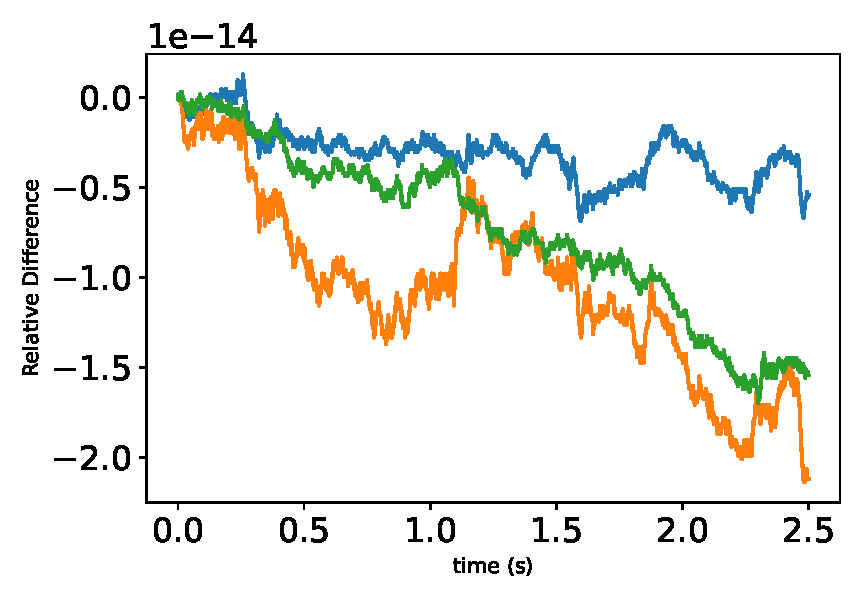
\includegraphics[width=0.8\textwidth]{AutoTeX/ChangeInOrbitalAngularMomentumGravity}}\caption{Change in Orbital Angular Momentum Gravity}\label{fig:ChangeInOrbitalAngularMomentumGravity}\end{figure}
\begin{figure}[htbp]\centerline{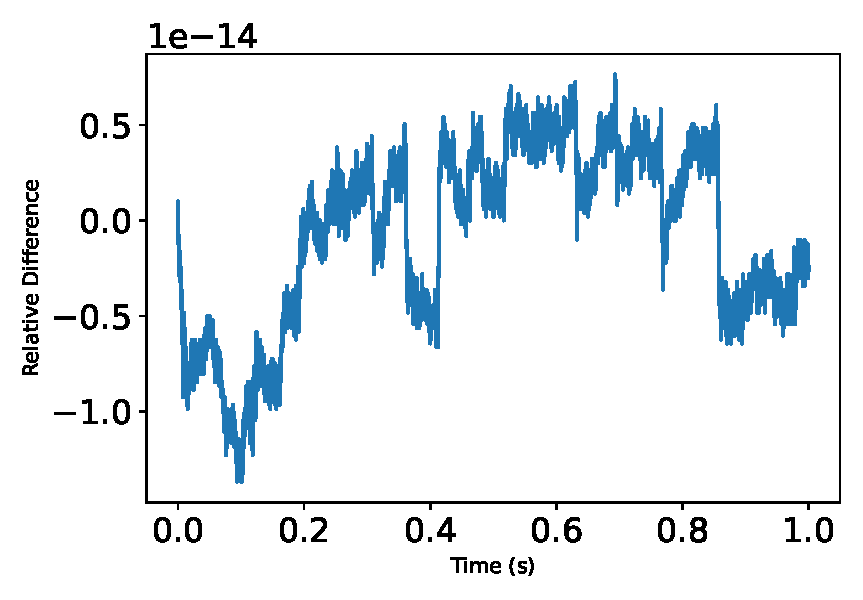
\includegraphics[width=0.8\textwidth]{AutoTeX/ChangeInOrbitalEnergyGravity}}\caption{Change in Orbital Energy Gravity}\label{fig:ChangeInOrbitalEnergyGravity}\end{figure}
\begin{figure}[htbp]\centerline{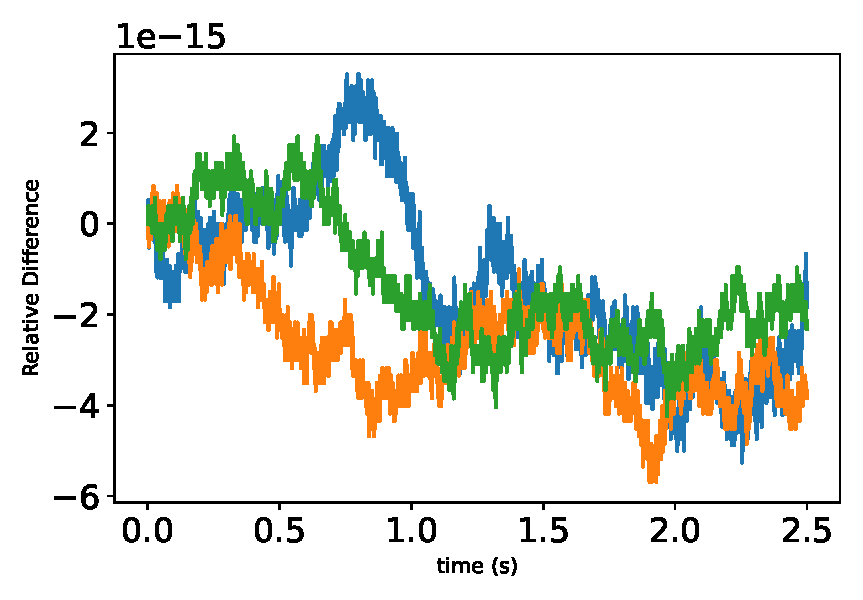
\includegraphics[width=0.8\textwidth]{AutoTeX/ChangeInRotationalAngularMomentumGravity}}\caption{Change In Rotational Angular Momentum with Gravity}\label{fig:ChangeInRotationalAngularMomentumGravity}\end{figure}
\begin{figure}[htbp]\centerline{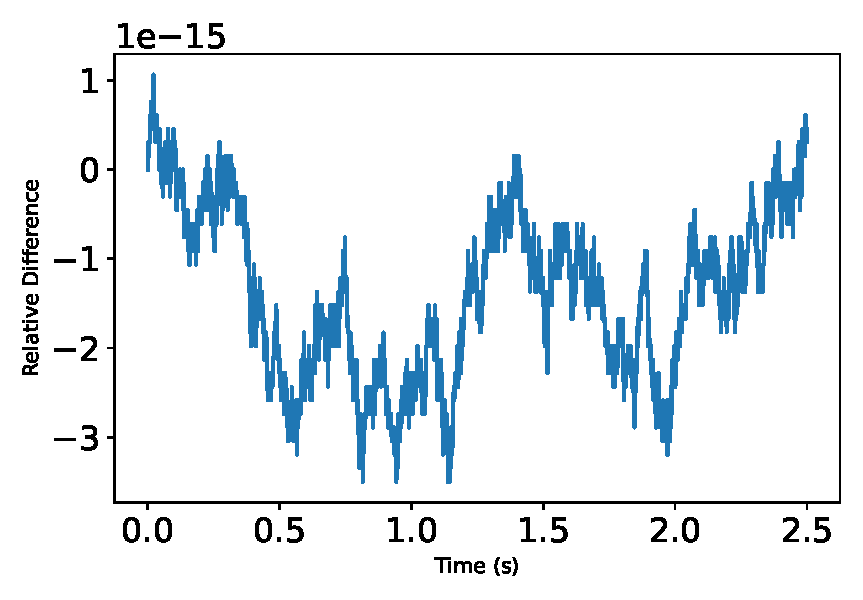
\includegraphics[width=0.8\textwidth]{AutoTeX/ChangeInRotationalEnergyGravity}}\caption{Change in Rotational Energy Gravity}\label{fig:ChangeInRotationalEnergyGravity}\end{figure}
\clearpage

\subsection{No Gravity with no damping scenario}
\begin{figure}[htbp]\centerline{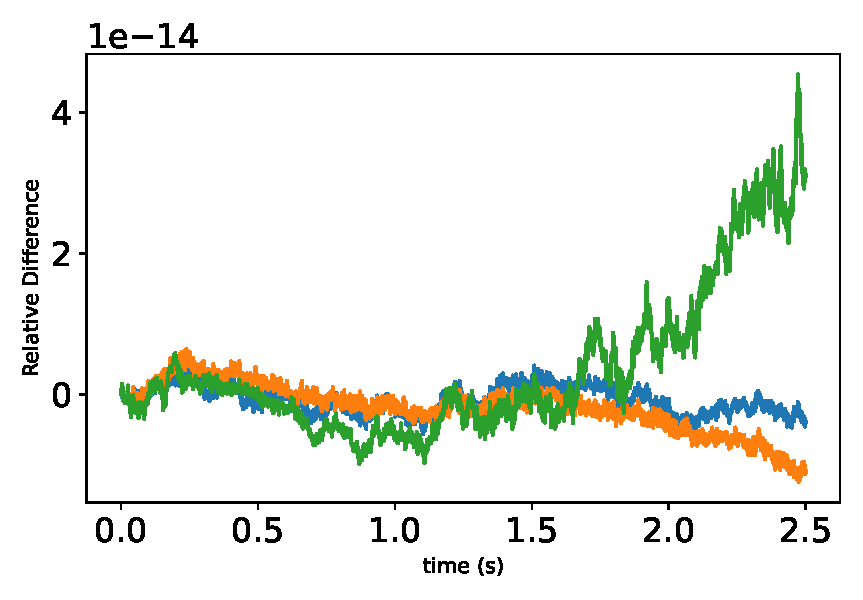
\includegraphics[width=0.8\textwidth]{AutoTeX/ChangeInOrbitalAngularMomentumNoGravity}}\caption{Change in Orbital Angular Momentum NoGravity}\label{fig:ChangeInOrbitalAngularMomentumNoGravity}\end{figure}
\begin{figure}[htbp]\centerline{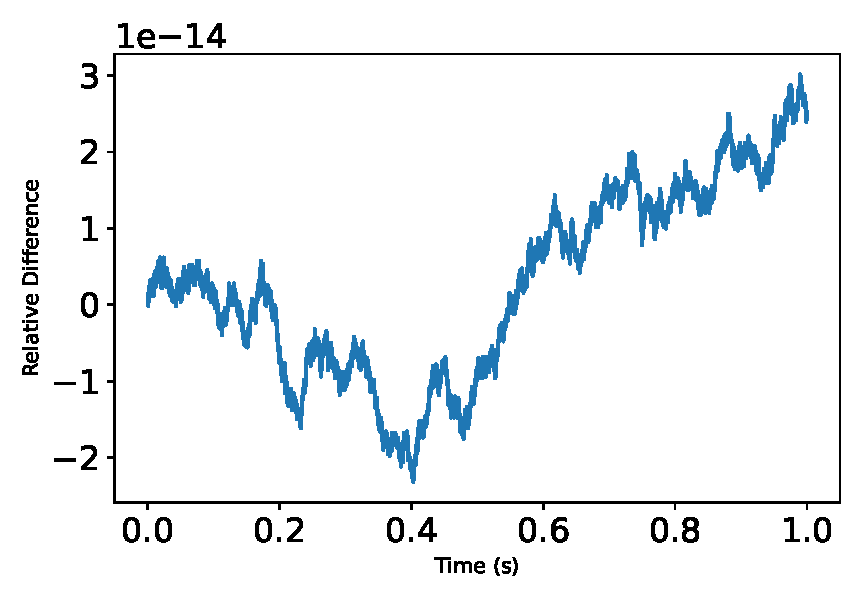
\includegraphics[width=0.8\textwidth]{AutoTeX/ChangeInOrbitalEnergyNoGravity}}\caption{Change in Orbital Energy No Gravity}\label{fig:ChangeInOrbitalEnergyNoGravity}\end{figure}
\begin{figure}[htbp]\centerline{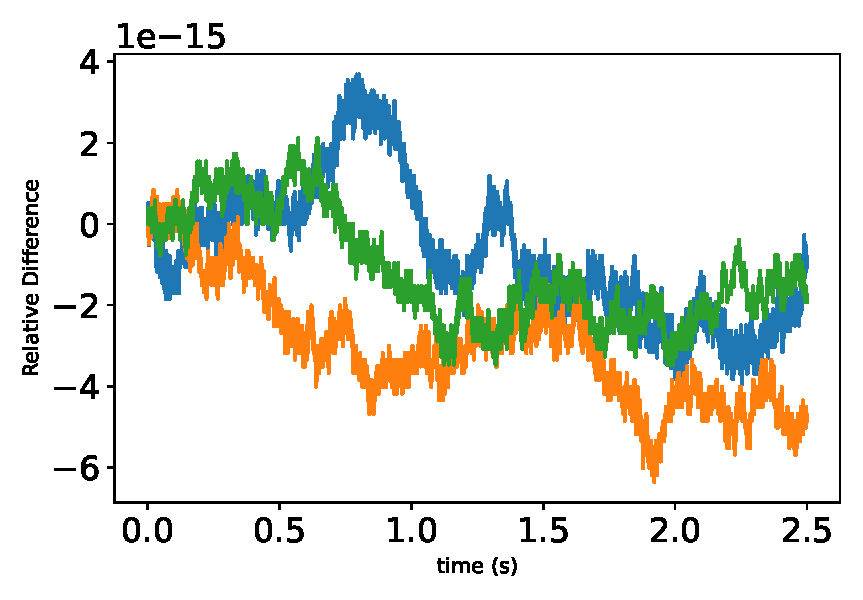
\includegraphics[width=0.8\textwidth]{AutoTeX/ChangeInRotationalAngularMomentumNoGravity}}\caption{Change in Rotational Angular Momentum NoGravity}\label{fig:ChangeInRotationalAngularMomentumNoGravity}\end{figure}
\begin{figure}[htbp]\centerline{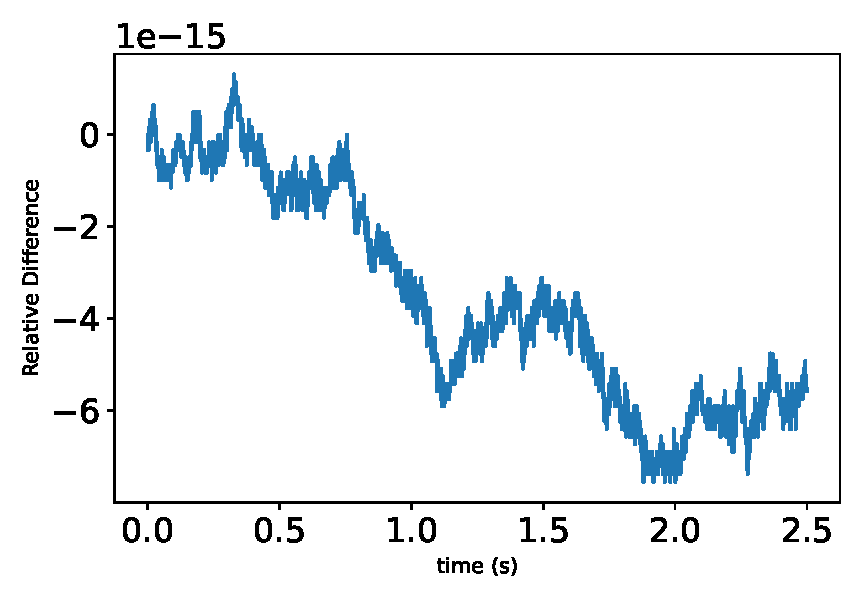
\includegraphics[width=0.8\textwidth]{AutoTeX/ChangeInRotationalEnergyNoGravity}}\caption{Change in Rotational Energy NoGravity}\label{fig:ChangeInRotationalEnergyNoGravity}\end{figure}
\clearpage
